\documentclass[11pt,a4paper]{article}   
\usepackage[cm]{fullpage}
\usepackage{polski}
\usepackage{mathtools}
\usepackage{amsmath}
\usepackage{amssymb}
\usepackage{color}
\usepackage{listings}
\usepackage[utf8]{inputenc}
\usepackage{tikz}
\usepackage{enumitem}
\usepackage[parfill]{parskip}
\setlength{\parindent}{0pt}

\newcommand\tab[1][1cm]{\hspace*{#1}}

%Definicje dla listingów
\definecolor{backcolor}{rgb}{0.95,0.95,0.92}
\lstdefinestyle{mystyle}{            
    numbers=left,
    backgroundcolor = \color{backcolor},
    tabsize = 2
}
\lstset{
	style=mystyle,
	mathescape=true,
	literate=
               {<-}{$\leftarrow{}$}{1}
               {->}{$\rightarrow{}$}{1},
    morekeywords={if,else,return,for, to}
}
%Definicje dla rysowania drzew
\usetikzlibrary{arrows}
\tikzset{
  treenode/.style = {circle, align=center, inner sep=0pt, text centered,
    font=\sffamily, black, draw=black, text width=1.5em, very thick}
}

\begin{document}                  

\title{Algorytmy Zaawansowane}
\author{Małgorzata Sobczak \and Jan Grzybowski \and Anna Witwicka}
\date{\today}

\maketitle 
                
\clearpage

\tableofcontents
\clearpage

\subsubsection{Notacja}
\(f,g,{\rm I\!N} \rightarrow {\rm I\!R}_+\)
\begin{itemize}
	\item \( g(n) = O(f(n))\) if \(\exists{c}>0\) \(\exists{n_0}\in {\rm I\!N} \) \(\forall{n} \leq n_0\) \(g(n) \geq c f(n)\)
    \item \( g(n) = \Omega(f(n))\) if \(\exists{c}>0\) \(\exists{n_0}\in {\rm I\!N} \) \(\forall{n} \leq n_0\) \(cf(n) \geq g(n)\)
    \item \( g(n) = \Theta(f(n))\) if \(\exists{c_1,c_2}>0\) \(\exists{n_0}\in {\rm I\!N} \) \(\forall{n} \leq n_0\) \(c_1 f(n)\geq g(n) \geq c_2 f(n)\)
\end{itemize}
\subsubsection{Algorytmy Zachłanne}
Idea: w każdym kroku algorytmu dokonuje lokalnie najlepszego wyboru, czyli wyboru, który w danym momencie wydaje się najkorzystniejszy.
\begin{itemize}
\item $S = \{ Z_1,...,Z_n \}$ - zbór zajęć używających tego samego zasobu (np. sali zajęć lub procesora) 
\item $s_i$ - czas rozpoczęcia zajęcia $z_i$
\item $t_i$ - czas zakończenia zajęcia $z_i$
\end{itemize}
zajęcia $z_i$ i $z_j$ są zgodne jeśli $<s_i,t_i)$ $\cup$ $<s_j,t_j) = \emptyset$ \\
Problem: Wybrać największej liczności zbiór $A \subset S$ parami zgodnych zajęć
\begin{center}
\begin{tabular}{ c | c | c | c | c | c | c }
  $i$ & $1$	& $2$ & $3$ & $4$ & $5$ & $6$ \\ \hline
  $s_i$ & 0	&  2  & 4 	& 7 & 1 & 7 \\ \hline
  $t_i$ & 4	&  6  & 7 	& 10 & 3 & 9 \\  
\end{tabular}
\end{center}
%\includegraphics[width=\textwidth]{UI_screens/Graph.png}

Algorytm zachłanny w każdym kroku wybierze zajęcie zgodne z każdym z już wybranych zajęć, które kończą się najwcześniej, żeby zostawić miejsce dla jak największej liczby kolejnych zajęć.\\
Sortujemy zajęcia niemalejąco względem czasów zakończenia (można to zrobić w czasie $O(n(logn))$.Dalej zakładamy, że $t_1 \leq t_2 \leq ... \leq t_n$

\begin{center}
\begin{tabular}{ c | c | c | c | c | c | c }
  $i$ & $1$	& $2$ & $3$ & $4$ & $5$ & $6$ \\ \hline
  $s_i$ & 1	&  0  &  2	&  4  &  7  & 7 \\ \hline
  $t_i$ & 3	&  4  &  6	&  7  &  9  & 10 \\  
\end{tabular}
\end{center}
\subsubsection{Algorytm}
gdzie s,t - wektory
\begin{enumerate}
	\item n $\leftarrow$ length(s)
    \item A $\leftarrow$ $\lbrace z_1 \rbrace$
    \item j $\leftarrow$ z
    \item for i $\leftarrow$ z to 1
    \item \tab if $s_i \geq t_j$ 
    \item \tab \tab A $\leftarrow$ A $\cup \lbrace z_j \rbrace$
    \item \tab \tab j $\leftarrow$ i
    \item return A
\end{enumerate}
Algorytm działa poprawnie tzn. zwraca zbiór zajęć parami zgodnych, bo dołącza zajęcie $z_i$ do zbioru razwiązań A tylko wtedy, gdy $s_i \geq t_j$, gdzie $t_j$ jest czasem zakończenia zajęcia wykonanego poprzednio.\\
\\
\underline{Tw.} Algorytm zawsze znajduje optymalne rozwiązania\\
Dowód Indukcja po n\\
\tab n = 1 ok.\\
\tab n $>$ 1\\
Pokazujemy najpierw, że istnieje rozwiązanie optymalne zawierające zajęcia $z_1$.\\
\\
Niech $A_1$ będzie dowolnym rozwiązaniem optymalnym i niech $\vert A_1\vert = l$\\
Jeśli $z_1 \in A_1$ to ok. \\
Niech w $z_1 \not\in A_1$ \\
Niech $z_k$ będzie zajęciem z $A_1$ o najmniejszym indeksie $\forall{j} \neq k, z_j \in A_1$ $s_j \geq t_n$ oraz $t_k \geq t_1$ zatem \\
$A_2 = (A_1 - \lbrace z_k\rbrace ) \cup \lbrace z_1 \rbrace $ też jest rozwiązaniem optymalnym \\
$A_2$ - rozwiązanie optymalne zawierające $z_1$\\
Rozważmy nasz problem dla zbioru $S' = \lbrace z_i \in S: s_i \geq t_i \rbrace$ Dla każdego $z_j \in A_2 - \lbrace z_1 \rbrace$ $z_j \in S'$, bo $S_j \geq t_1$, bo $A_2$ jest rozwiązaniem dla $S$. Pokażemy, że $A_2 - \lbrace z_1 \rbrace$ jest rozwiązaniem optymalnym problemu dla $S'$. Gdyby istniało rozwiązanie $B$ dla $S'$ liczniejsze od $A_2 - \lbrace z_1 \rbrace$, to $\lbrace z_1 \rbrace \cup B$ było by rozwiązaniem problemu dla $S$ liczniejszym od $A_2$. \\
$\vert S' \vert \leq \vert S \vert$\\
Z założenia indukcyjnego algorytm znajduje rozwiązanie optymalne $B'$ dla $S'$ o liczności $\vert A_2 \vert - 1 = l - 1$\\
Algorytm znajduje dla zbioru $S$ rozwiązanie $\lbrace z_1 \rbrace \cup B'$ o liczności $\vert \lbrace z_1 \rbrace \cup B' \vert = 1 + l - 1 = l$, więc $\lbrace z_1 \rbrace \cup B'$, jest rozwiązaniem optymalnym.\\
\\
\textbf{Złożoność obliczeniowa}\\
linia 1 \tab $O(n)$\\
linia 2,3 \tab $O(n)$\\
pętla w linii 4 wykonuje się $O(n)$ razy\\
\tab wykonanie tej pętli zajmuje $O(1)$ czasu\\
$\Theta(n)$ jeśli zajęcie są posortowane względem czasu zakończenia \\
\underline{$O(nlogn)$ złożoność całego rozwiązania.}



\subsection{Kody Huffmann'a}
Zwykle znaki są reprezentowane za pomocą 8 bitów (np. ASCII). Ponieważ jednak częstości wystąpień znaków różnią się, opłaca się reprezentować częściej występujące znaki za pomocą krótszych ciągów bitów, a rzadziej  występujące za pomocą dłuższych.\\

Dążymy do użycia jak najmniejszej ilości bitów.\\

\textbf{Przykład:} W pliku występuje 58 znaków a, e, i, s, t, r, n\\
\begin{center}
\begin{tabular}{ l | c | c | c | c | c | c | c }
  	 										& $a$	& $e$ 	& $i$ 	& $s$ 	& $t$ 	& $r$ 	& $n$ 	\\ \hline
  częstość wystąpień 						& 10	&  15  	& 12	&  3  	&  4	&  13	&  1 	\\ \hline
  kod 1 (stała długość słowa kodowego) 		& 000 	& 001 	& 010	& 011 	& 100	& 101	& 110 	\\ \hline
  kod 2 (zmienna długość słowa kodowego) 	& 001 	& 01 	& 10	& 00000 & 0001	& 11	& 00001 \\ \hline
  kod 3 (zmienna długość słowa kodowego) 	& 001 	& 01 	& 10	& 00010 & 0001	& 11	& 00001 \\  
\end{tabular}
\end{center}

Przy stałej długości słów kodowych zakodowanych plik ma: $58*3=174$ bity. \\
Przy zmiennej długości słów kodowych zakodowany plik ma: $3 \cdot 10+2 \cdot 15+2 \cdot 12+5 \cdot 3+4 \cdot 4+2 \cdot 13+5 \cdot 1 = 146$ bitów. Oszczędzamy około 15$\%$ .

Przy kodowaniu ze zmienną długością słów kodowych chcemy, żeby spełniony był warunek, że żadne słowo nie jest prefiksem (początkiem) innego słowa. Takie kody nazywamy prefiksowymi.

\textbf{Słowo 0001001 można zdekodować za pomocą kodu 3. na dwa sposoby:}
\begin{itemize}
	\item 00010 01 se
	\item 0001 001 ta 
\end{itemize}
Tutaj 0001 jest prefiksem słowa 00010 czyli kod t jest prefiksem kodu s. \textbf{Zatem kod 3. nie jest kodem prefiksowym.}

\textbf{Reprezentacja kodów za pomocą drzew}\\
\textbf{Kod 1}
%\includegraphics[width=\textwidth]{UI_screens/Graph.png}

\textbf{Kod 3}
%\includegraphics[width=\textwidth]{UI_screens/Graph.png}

\textbf{Kod 2}
%\includegraphics[width=\textwidth]{UI_screens/Graph.png} 

\paragraph{Stwierdzenie} Żadne słowo nie jest prefiksem innego słowa wtedy i tylko wtedy, gdy w drzewie reprezentującym ten kod wszystkie znaki są liśćmi.
\begin{center}
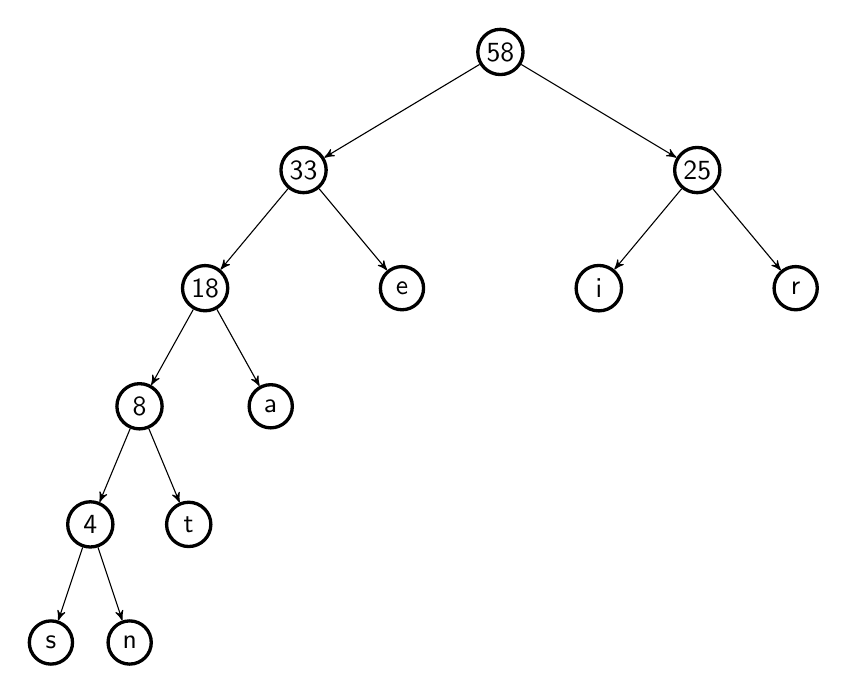
\begin{tikzpicture}[->,>=stealth',level/.style={sibling distance = 5cm/#1,
  level distance = 1.5cm}] 
\node [treenode] {58}
    child{ node [treenode] {33} 
        child{ node [treenode] {18} 
        	child{ node [treenode] {8} 
				child{ node [treenode] {4} 
					child{ node [treenode] (s) {s} }
					child{ node [treenode] (n) {n} } 				
				}
				child{ node [treenode] (t) {t} }            	
            }
			child{ node [treenode] (a) {a} }	
		}  
		child{ node [treenode] (e) {e} }
    }
    child{ node [treenode] {25}
            child{ node [treenode] (i) {i} }
            child{ node [treenode] (r) {r} }
	}
; 
\end{tikzpicture}
\end{center}

Etykietujemy wierzchołki wewnętrzne drzewa w taki sposób, aby każdy wierzchołek $x$ otrzymywał etykietę będącą sumą ilości wystąpień znaków będących liśćmi w poddrzewie o korzeniu $x$. 

Niech:
\begin{itemize}
\item $C$ będzie alfabetem
\item $f(c)$ liczbą występowania znaku $c$
\item $d_T(c)$ głębokością liścia $c$ w drzewie 
\item $T$ (równą długości słowa kodowego reprezentującego $c$)
\end{itemize}  Liczba bitów potrzebnych do zakodowania całego pliku wynosi 
$$B(T) = \sum_{c \in C} f(c) \cdot d_T(c)$$

Kod prefiksowy zdefiniowany przez drzewo $T$ jest optymalny jeśli liczba $B(T)$ jest najmniejsza możliwa.

Drzewo ukorzenione jest \textbf{binarne} jeśli każdy wierzchołek, nie będący liściem, ma co najwyżej 2 dzieci.

Drzewo binarne jest \textbf{regularne} jeśli każdy wewnętrzny wierzchołek ma dokładnie 2 dzieci.

\paragraph{Twierdzenie}{Drzewo binarne reprezentujące kod optymalny jest regularne.}

\paragraph{Dowód\\}{}
Załóżmy, że:
\begin{itemize}
\item $T$ - Drzewo reprezentujące optymalny kod prefiksowy. Przypuśćmy, że $T$ nie jest regularne. Wtedy istnieje w T wewnętrzny (nie będący korzeniem ani liściem) wierzchołek z dokładnie jednym dzieckiem.
\item $w$ - pojedyncze dziecko
\item $v$ - rodzic $w$, nie będący korzeniem drzewa.
\item $u$ - rodzic $v$
\end{itemize}
%Ilustracja

Tworzymy nowe drzewo $T'$ poprzez usunięcie $v$ z drzewa i dodanie krawędzi $uw$ o ile $v$ nie jest korzeniem.
Jeżeli $B(T) < B(T')$ zachodzi sprzeczność, ponieważ $T$ miało być drzewem optymalnym.

\subsubsection{Algorytm tworzenia drzewa reprezentującego optymalny kod prefiksowy}
Algorytm tworzenia drzewa reprezentującego optymalny kod prefiksowy dla $(C,f)$. 

Zaczynamy od $|C|$ liści, następnie wykonujemy $|C|-1$ operacji scalania zaczynając od najrzadziej występujących znaków (będą one leżały najgłębiej w drzewie). Będziemy używać kolejki priorytetowej z klasami $f(c)$. 

Kolejkę priorytetową można zaimplementować jako kopiec binarny. Wtedy poszczególne operacje będą miały następujący koszt:
\begin{itemize}
\item insert $O(\log n)$ 
\item extract\_min $O(\log n)$
\item create $O(n)$
\end{itemize}
gdzie $n$ będzie liczbą elementów w kolejce.

\paragraph{Przykład}
\begin{enumerate}
\item n:1 s:3 t:4 a:10 i:12 r:13 e:15
%Ilustracja
\end{enumerate}

\subsubsection{Algorytm Huffmana}
Załóżmy istnienie funkcji $left(z), right(z)$ - zwracające dzieci wierzchołka $z$.
\begin{lstlisting}[caption={Huffman(C,F)}]
n <- |C|
Q <- create_queue(C)
for i <- 1 to n-1
	z <- create_new_node
	x <- left(z) <- extract_min(Q)
	y <- right(x) <- extract_min(Q)
	f(z) <- f(x) + f(y)
	insert(Q,z)
\end{lstlisting}

Algorytm konstruuje drzewa binarne.

\textbf{Złożoność algorytmu Huffmana:}
\begin{lstlisting}
$O(1)$
$O(1)$
$n-1$ razy
	wnetrze petli $\log n$ razy
\end{lstlisting}
\underline{Ostateczna złożoność algorytmu to $O(n \log n)$}

\subsubsection{Twierdzenie o poprawności Algorytmu Huffmana}
\textbf{Lemat 1.} Niech $x$ i $y$ będą parą znaków z $C$ o najmniejszej liczbie wystąpień. Istnieje optymalny kod prefiksowy, w którym kody dla $x$ i $y$ mają tę samą długość i różnią się tylko wartością ostatniego bitu.

\textbf{Dowód} Znajdujemy drzewo reprezentujące kod optymalny, w którym liście reprezentujące $x$ i $y$ są bliźniakami i są najgłębiej w drzewie. Niech $T$ będzie drzewem reprezentującym kod optymalny i niech $a$ i $b$ będą liśćmi bliźniakami najgłębiej w T. 
Bez straty ogólności możemy założyć:
$$ f(x) \leq f(y); f(a) \leq f(b) $$
ponieważ $f(x)$ i $f(y)$ są najmniejszymi liczbami:
$$ f(x) \leq f(a); f(y) \leq f(b) $$
Niech $T'$ będzie drzewem powstałym z $T$ przez zamianę miejscami $x$ z $a$
$$ B(T) - B(T') = \sum_{c \in C} f(c) \cdot d_T(c) - \sum_{c \in C} f(c) \cdot d_{T'}(c) $$
$$ = f(x) \cdot d_T(x) + f(a) \cdot d_T(a) - f(x) \cdot d_{T'}(x) - f(a) \cdot d_{T'}(a) $$
$$ = f(a) \cdot (d_T(a) - d_T(x)) + f(x) \cdot (d_T(x) - d_T(a)) $$ 
$$ = (f(a) + f(x)) \cdot (d_T(a) - d_T(x)) \geq 0$$
Zatem $B(T') \leq B(T)$ a jednocześnie $T$ jest optymalne. Zatem $B(T') = B(T)$ więc $T'$ też jest drzewem reprezentującym kod optymalny. Analogicznie zamieniamy $y$ z $b$.

\paragraph{Z lematu 1.} {wynika, że możemy zacząć kodowanie optymalnego kodu prefiksowego od dwóch znaków najrzadziej występujących. Zachłanność wyboru polega na wybieraniu obiektów o najmniejszej częstości.}

\paragraph{Lemat 2.} {$A$ - alfabet. Niech $x$ i $y$ będą parą znaków z $A$ o  najmniejszej częstości. 
\\ Niech $A'= (A - \{x,y\}) \cup \{z\}$ gdzie $z \not\in A$. 
\\ Funkcję $f$ definiujemy jak dla $A$ a dodatkowo $f(z) = f(x) + f(y)$.

$T'$ - drzewo reprezentujące kod optymalny dla $A'$

$T$ - drzewo powstałe z $T'$ przez zastąpienie liścia $z$ wierzchołkiem wewnętrznym z dziećmi $x$ i $y$.

Drzewo $T$ jest drzewem reprezentującym kod optymalny dla A.}

\paragraph{Dowód} Dla $c \in A - \{x,y\}$ zachodzi $d_T(c) = d_{T'}(c)$ oraz $d_T(x) = d_T(y) = d_{T'}(z)+1$, stąd 

$$B(T) = \sum_{c \in A}(f(c) \cdot d_T(c)) = \sum_{c \in A-\{x,y\}}f(c) \cdot d_T(c) + f(x) \cdot d_T(x) + f(y) \cdot d_T(y)$$

$$ = \sum_{c \in A-\{x,y\}}f(c) \cdot d_T(c) + (d_{T'}(z) +1) \cdot (f(x) + f(y)) = \sum_{c \in A-\{x,y\}}f(c) \cdot d_T(c) + f(z) \cdot d_{T'}(z) + f(x)+ f(y)$$

$$ = \sum_{c \in A'}f(c) \cdot d_{T'}(c) + f(x) + f(y) = B(T') + f(x) + f(y) \implies B(T') = B(T) - f(x) - f(y)$$

Przypuśćmy, że $T$ nie reprezentuje optymalnego kodu dla A. 

Istnieje $T''$ reprezentujące kod optymalny dla A i $B(T'') < B(T)$. Na mocy \textbf{lematu 1.} możemy wybrać $T''$ tak, aby $x$ i $y$ były w $T''$ bliźniakami najgłębiej położonymi w drzewie. 

Niech $T'''$ będzie drzewem powstałym z $T''$ przez wyrzucenie $x$ i $y$ i dodanie $z$ oraz $f(z) = f(x) + f(y)$. $T'''$ jest drzewem reprezentującym pewien kod prefiksowy dla $A'$. 

Analogicznie możemy pokazać, że $B(T''') = B(T'') - f(x) - f(y)$. Wtedy $B(T''') = B(T'') - f(x) - f(y) < B(T) - f(x) - f(y) = B(T')$. 

Otrzymujemy sprzeczność $B(T''') < B(T')$ ponieważ $T'$ miało reprezentować kod optymalny dla $A'$.

\paragraph{Twierdzenie} Algorytm Huffmana zawsze znajduje optymalny kod prefiksowy.
\paragraph{Dowód} {Indukcja po $n = |C|$}

Dla $n = 1,2$ twierdzenie jest prawdziwe.

Dla $n > 2$:

Po pierwszym scaleniu otrzymujemy alfabet $C' = (C - {x,y}) \cup \{z\}$, funkcję $f$ taką, że $f(z) = f(z) + f(y)$, a dla pozostałych argumentów jest zdefiniowana jak przed scaleniem. $x$ i $y$ są najrzadziej występującymi znakami w C. 
$$|C'| = |C| - 1$$
Z założenia indukcyjnego algorytmu znajdującego drzewo $T'$ reprezentujące kod optymalny dla $C'$. Algorytm znajduje dla $C$ drzewo $T$ powstałe z $T'$ przez zastąpienie liścia $z$ wierzchołkiem wewnętrznym z dziećmi $x$i $y$ z \textbf{lematu 2.} $T$ reprezentuje optymalny kod prefiksowy dla $C$






\subsection{Prosty problem szeregowania zadań}
\subsection{Prosty problem szeregowania zadań}
\subsubsection{Opis problemu}
Instancja problemu składa się z:
\begin{itemize}
	\item Zbioru zadań do wykonania $Z= \{ Z_1,...,Z_n \}$
    \item Czasów wykonania zadań $t = \{ t_1,...,t_n\}$
\end{itemize}
Rozpoczęte zadnie nie może być przerwane.
Jak uszeregować $Z$, aby średni czas ukończenia był najmniejszy?

\subsubsection{Przykład dla 1 procesora}
\begin{center}
\begin{tabular}{ c | c | c | c | c }
  $z$ & $z_1$	& $z_2$ & $z_3$ & $z_4$ \\ \hline
  $t$ & 15 		&  8 	& 3 	& 10 \\ 
\end{tabular}
\end{center}
Średni czas ukończenia zadania dla kolejności $z_1, z_2, z_3, z_4$:
$\frac{15+(15+8)+(15+8+3)+(15+8+3+10)}{4}= 25$ 


Średni czas ukończenia zadania dla kolejności $z_3, z_2, z_4, z_1$:
$\frac{3+(3+8)+(3+8+10)+(3+8+10+15)}{4} = 17\frac{3}{4}$ 


\textbf{Wniosek:} wykonujemy zadania sortując rosnąco po $t$.

\subsubsection{Przykład dla 3 procesorów}
Przydzielamy kolejne zadania pierwszemu wolnemu procesorowi:
\begin{center}
\begin{tabular}{ c | c | c | c | c | c | c | c | c | c } 
  $z$ 	& $z_1$	& $z_2$ & $z_3$ & $z_4$	& $z_5$	& $z_6$ & $z_7$ & $z_8$	& $z_9$ \\ \hline
  $t$ 	& 3		& 5		& 6		& 10	& 11	& 14	& 15	& 18	& 20 \\ 
\end{tabular}
\end{center}

\begin{center}
\begin{tabular}{ c | c | c | c }
  CPU1 & $z_1$ & $z_4$ & $z_7$ \\ \hline
  CPU2 & $z_2$ & $z_5$ & $z_8$ \\ \hline
  CPU3 & $z_3$ & $z_6$ & $z_9$ \\
\end{tabular}
\end{center}

\subsubsection{Dowód}
Przy uszeregowaniu $z_{i_1} ,..., z_{i_n}$ suma czasów ukończenia wynosi:
\begin{itemize}
	\item \textbf{dla 1 procesora:}
	\[ \sum_{j=1}^{n} \sum_{k=1}^{j} t_{i_k} = t_{i_1} + (t_{i_1}+ t_{i_2}) + ... + (t_{i_1} + ... + t_{i_n}) = n \cdot t_{i_1} + ... + 1 \cdot t_{i_n} = \sum_{j=1}^{n} (n+1-j) t_{i_j}  \]
    \item \textbf{dla 3 procesorów:}
	$$ t_{i_1} + t_{i_2} + t_{i_3} + (t_{i_1}+ t_{i_4}) + (t_{i_2}+ t_{i_5}) + (t_{i_3}+ t_{i_6}) + ... + (t_{i_1} + ... + t_{i_{n-2}}) + (t_{i_2} + ... + t_{i_{n-1}}) + (t_{i_3} + ... + t_{i_n}) $$
	$$ = \frac{n}{3} (t_{i_1} + t_{i_2} + t_{i_3}) + \frac{n-1}{3} (t_{i_4} + t_{i_5} + t_{i_6}) + ... + 1 (t_{i_{n-2}} + t_{i_{n-1}} + t_{i_{n}}) $$
	$$ = \sum_{j=1}^{n} (\frac{n}{3} - \lfloor\frac{j-1}{3}\rfloor) t_{i_j}$$
	$$ = \sum_{j=1}^{n} \lceil \frac{n + 1 -j}{3} \rceil t_{i_j}  $$
	\end{itemize}

\paragraph{Lemat:} Niech $A_1 \geq A_2 \geq ... \geq A_n$. Dla dowolnej permutacji $\pi = (i_1, ..., i_n)$ zbioru ${1,...n}$ niech $$f(\pi) = \sum_{j=1}^{n} A_j \cdot t_{i_j}$$ $f(\pi)$ jest najmniejsze dla permutacji $\pi$ takich, że $t_{i_1} \leq t_{i_2} \leq ... \leq t_{i_n}$.

\paragraph{Dowód:} Niech $\pi$ będzie permutacja minimalizującą $f(\pi)$. Przypuśćmy, że dla pewnych $k$ i $l$ takich, że $k<l$ i $t_{i_k} > t_{i_l}$. Niech $\pi'$ będzie permutacją powstałą z $\pi$ za pomocą zamiany miejscami $i_k$ z $i_l$ tzn. $i'_j = i_j$ dla $j\neq k,l$ i $i'_k = i_j$ $i'_j = i_k$. \\
Wtedy
$$ f(\pi) - f(\pi') = \sum_{j=1}^{n} A_j \cdot t_{i_j} - \sum_{j=1}^{n} A_j  \cdot t_{i'_j} $$
$$ = A_k \cdot t_{i_k} - A_k \cdot t_{i'_k} + A_l \cdot t_{i_l} - A_l \cdot t_{i'_l} $$
$$ =A_k(t_{i_k} - t_{i_l}) - A_l(t_{i_k} - t_{i_l}) = (A_k - A_l)(t_{i_k} - t_{i_l}) \geq 0 $$

$f(\pi) \geq f(\pi')$ więc $f(\pi) \geq f(\pi')$ bo $\pi$ minimalizuje f. 
Po pewnej liczbie takich zamian otrzymujemy $\pi$ - permutację minimalizującą f i taką, że $t_{i_1} \leq ... \leq t_{i_n}$ .
\\
\textbf{Wnioski:} Oba algorytmy szeregowania są poprawne.




\subsection{Matroidy}
\subsubsection{Definicja}
Matroidem nazywamy strukturę $M = (S,\mathbb{A})$ taką, że:
\begin{enumerate}
	\item $S$ jest niepustym zbiorem skończonym
	\item $\mathbb{A} \subset 2^S$
	\item $\forall A,B \subset S$   $A \in \mathbb{A} \land B \subset A \implies B \in \mathbb{A}$
	\item $\forall A,B \subset S$ 	$A,B \in \mathbb{A} \land \|B\| < \|A\| \implies \exists x \in B - A A \cup \{x\} \in \mathbb{A} $ (warunek wymiany)
\end{enumerate}
$\mathbb{A}$ nazywamy rodziną zbiorów niezależnych.
\\

\textbf{Przykłady:} 
\begin{enumerate}
	\item $S$ - zbiór wierszy macierzy \\
	$M = (S,\mathbb{A})$;
	$A \subset S$;
	$A\in\mathbb{A}$ jeśli wiersze z $A$ są liniowo niezależne.

	\item $S$ - zbiór krawędzi w grafie \\
	$\mathbb{A}$ - zbiory krawędzi indukujące lasy \\
	$M = (E,\mathbb{A})$;  
	$G = (V,E)$;     
	$\mathbb{A} = \{F \subset E : G(F)$ jest acykliczny$\}$
\end{enumerate}

\subsubsection{Problem}
$M = (S,\mathbb{A})$\\
$w:S \rightarrow (0,\infty)$ funkcja wagi \\
$w:S^2 \rightarrow (0, \infty) = \sum{x\in A} w(x)$ \\
Należy znaleźć zbiór niezależny $a \in \mathbb{A}$ o maksymalnej sumie wag.
\begin{lstlisting}[caption={Greedy(M,w)}]
$\mathbb{A} = \emptyset$
uporzadkuj S niemalejaco wzgledem wag $w(x_1) \geq w(x_2) \geq ... \geq w(x_n)$
for $i$ = 1 to n
	if $A \cup \{x_i\} \in \mathbb{A}$
		$A = A \cup \{x_i\}$
\end{lstlisting}

\textbf{Tw. (Rado Endmonds)} Algorytm Greedy znajduje zbiór niezależny Matroidu o maksymalnej wadze. \\
\begin{lstlisting}

$O(n \log n)$
$n$
$f(n)$ - czas sprawdzenia warunku w linii 4.

\end{lstlisting}

\textbf{Złożoność Greedy} $O(n \log n + n \cdot f(n)$


\subsection{Problem szeregowania zadań}
\subsection{Problem szeregowania zadań}
\subsubsection{Definicja problemu}
\begin{itemize}
\item $S = {z_1, ... ,z_n}$ - zbiór zadań każde o $t_{i_j}=1$ 
\item $d_1, ... , d_n$,  $d_i \in \{1,...,n\}$ - deadline'y zadań 
\item $w_1, ... , w_n$, $w_i \in \{1,...,n\}$ - kary za nie wykonanie zadania $z_i$ do chwili $t=d_i$ \\
\end{itemize}
W problemie szeregowania zadań szukamy permutacji zadań z najmniejszą łączną karą. 

Jeżeli zadanie zostanie ukończone po deadlinie, nazywamy je \textbf{spóźnionym}, w przeciwnym przypadku zadanie jest nazywane \textbf{terminowym}. 

\paragraph{Lemat 1.}{Każde uszeregowanie można doprowadzić do uszeregowania o takiej samej sumie kar, w którym:}
\begin{itemize}
	\item zadania terminowe poprzedzają opóźnione,
	\item zadania terminowe występują w kolejności niemalejącej względem deadlinów.
\end{itemize}  

\textbf{Dowód}
\begin{enumerate}
	\item{Niech: 
	\begin{itemize}
		\item $z_i$ będzie spóźnione, ukończone w chwili $l_i$ $(l_i > d_i)$.
		\item $z_j$ będzie terminowe, ukończone w chwili $l_j$ $(l_j \leq d_j)$.
		\item $z_i$ jest wykonywane przed $z_j$ ($l_i < l_j$)
	\end{itemize}
	Po zamianie $z_j$ z $z_i$:
	\begin{itemize}
		\item $z_i$ jest ukończone w chwili $l_j > l_i > d_i$, nadal opóźnione.
		\item $z_j$ jest ukończone w chwili $l_i \leq l_j \leq d_j$, nadal terminowe.
	\end{itemize}
	}
	
	\item{Niech:
	\begin{itemize}
		\item $z_i$ będzie terminowe, ukończone w chwili $l_i$ $(l_i \leq d_i)$.
		\item $z_j$ będzie terminowe, ukończone w chwili $l_j$ $(l_j \leq d_j)$.
		\item $z_i$ jest wykonywane przed $z_j$ ($l_i < l_j$)
		\item $d_j < d_i$
	\end{itemize}
	Po zamianie $z_j$ z $z_i$:
	\begin{itemize}
		\item $z_i$ jest ukończone w chwili $l_j \leq l_i \leq d_i$, nadal terminowe.
		\item $z_j$ jest ukończone w chwili $l_i \leq l_j \leq d_j$, nadal terminowe.
	\end{itemize}
	}
\end{enumerate}
Zatem dokonują zamian z punktu 1. lub punktu 2. możemy przekształcić uszeregowanie w inne o takiej samej sumie kar takie, które spełnia warunki lematu.
\\

\textbf{Pojęcia dodatkowe do lematu 2.}

Zbiór zadań $A \subset S$ nazywamy \textbf{niezależnym}, jeśli daje się go uszeregować tak, że wszystkie zadania są terminowe. 

Definiujemy $N_t(A) = |\{z_i \in A : d_i \leq t \}|$ - liczba zadań których $d$ nie jest większe od $t$. 

\paragraph{Lemat 2.} 
Dla każdego $A \subset S$ następujące warunki są równoważne:
\begin{enumerate}
	\item $A$ jest niezależne
	\item $N_t(A) \leq t$ dla $t = 1,...,n$
	\item jeśli zadania w $A$ są uszeregowane niemalejąco względem deadlinów, to żadne zadanie nie jest opóźnione.
\end{enumerate}  

\textbf{Dowód}
\begin{itemize}
	\item{ $1 \implies 2$: 
	Jeśli $N_t(A) > t$ dla pewnego $t$ to do chwili $t$ trzeba by ukończyć więcej niż $t$ zadań. W takiej sytuacji nie da się uszeregować zadań z $A$ tak, aby wszystkie były terminowe, więc $A$ nie jest niezależne.}
	\item{ $2 \implies 3$: 
	Szeregujemy zadania w $A$ niemalejąco względem deadlinów. Gdyby pewne zadanie $z_t$ w tym uszeregowaniu było spóźnione i zakończone w chwili $l_t$ to byłoby co najmniej $l_t$ zadań o deadlinie $\leq d_t$. $z_t$ jest spóźnione, więc $l_t > d_t$.}
	\item{ $3 \implies 1$: Z definicji zbioru niezależnego.}
\end{itemize}

\subsubsection{Algorytm rozwiązujący problem szeregowania zadań}
Szukamy takiego podzbioru niezależnego $A$ tak, aby suma kar dla elementów spoza $A$ była jak najmniejsza. $\sum_{z_i \not\in A} w_i = \sum_{z_i \in S} w_i - \sum_{z_i \in A} w_i$ co oznacza maksymalizację sumy $\sum_{z_i \in A} w_i$. 

Jeżeli nasz problem ma strukturę matroidu to możemy rozwiązać go algorytmem zachłannym (Patrz tw. RadoEndmonds).

\textbf{Twierdzenie} 

$S$ - zbiór zadań i jednostkowych czasach wykonania 

$\mathbb{A}$ - rodzina zbiorów niezależnych 

$(S,\mathbb{A})$ jest matroidem 


\textbf{Dowód}
\begin{enumerate}
	\item $S$ jest niepustym skończonym zbiorem
	\item $\mathbb{A} \subset 2^S$
	\item $A\in\mathbb{A}$, $B \subset A$ 
	
	Uszeregowanie B powstałe z właściwego uszeregowania $A$ przez wykreślenie z uszeregowania elementów spoza $B$. Jeżeli wszystkie zadania z uszeregowania $A$ były terminowe to w $B$ tak samo wszystkie zadania będą terminowe.

	\item $A,B \in \mathbb{A}, |B| > |A|$

	Za pomocą $k, 0\leq k \leq n$ oznaczamy największe $t$ takie, że $N_t(B) \leq N_t(A)$. $k$ jest dobrze zdefiniowane, ponieważ $N_0(B) = 0 = N_0(A)$. $N_n(B) = |B| >  |A| = N_n(A)$, zatem  $0\leq k \leq n$. 
	
$\begin{drcases}
	N_{k+1}(B) > N_{k+1}(A) \\
	N_k(B) \leq N_k(A)
\end{drcases}$ istnieje zadanie $x \in B - A$ o deadlinie równym $k+1$

Niech $A' = A \cup \{x\}$. Pokażemy, że $A'$ jest niezależny używając \textbf{Lematu 2}. 
\begin{itemize}
	\item Ponieważ $A$ jest niezależne, dla $1 \leq t \leq k$ mamy $N_t(A') = N_t(A) \leq t$
	\item Ponieważ $B$ jest niezależne, dla $k+1 \leq t \leq n$ mamy $N_t(A') = N_t(A)+1 \leq N_t(B) \leq t$
\end{itemize}
\end{enumerate}
Zatem $(S,\mathbb{A})$ jest matroidem. Z Tw. Rado-Edmondsa wiemy, że algorytm Greedy zwraca optymalne rozwiązanie. Dla problemu szeregowania zadań linijkę 4. w algorytmie możemy przerobić, tak aby działała w czasie $O(n)$. Zatem złożoność całego algorytmu wynosi $O(n^2)$.

\subsubsection{Przykład działania algorytmu Greedy}
\begin{center}
\begin{tabular}{ c | c | c | c | c | c | c | c | c } 
  	 	& $z_1$	& $z_2$ & $z_3$ & $z_4$	& $z_5$	& $z_6$ & $z_7$ & $z_8$	\\ \hline
  $d_i$	& 3		& 2		& 2		& 3		& 1		& 4		& 6		& 5		\\ \hline
  $w_i$	& 80	& 70	& 60	& 50	& 40	& 30	& 20	& 10	\\ 
\end{tabular}
\end{center}
\begin{enumerate}
	\item $\{ z_1 \}$
	\item $\{ z_2, z_1, \}$
	\item $\{ z_3, z_2, z_1, \}$
	\item $\{ z_3, z_2, z_1, \}$
	\item $\{ z_3, z_2, z_1, \}$
	\item $\{ z_3, z_2, z_1, z_6, \}$
	\item $\{ z_3, z_2, z_1, z_6, z_7 \}$
	\item $\{ z_3, z_2, z_1, z_6, z_8, z_7 \}$
\end{enumerate}



\section{Programowanie Dynamiczne}
\section{Programowanie Dynamiczne}
Czasami, gdy próbujemy rozwiązać problem formułą rekurencyjną otrzymujemy bardzo wolny algorytm o złożoności wykładniczej. Najczęściej do takich sytuacji dochodzi, gdy liczymy te same rzeczy wielokrotnie.

\subsection{Liczby Fibonacciego}
$$ F(n) = \begin{cases}
	F(0) = F(1) = 1 \\
	F(n) = F(n-1) + F(n-2)
\end{cases}$$
\subsubsection{Implementacja rekurencyjna} 
\begin{lstlisting}[caption={FIBR(n) - rekurencyjny algorytm liczący n-tą liczbę Fibonacciego}]
if $n \leq 1$ return 1
return FIBR(n-1) + FIBR(n-2)
\end{lstlisting}
Ilość wywołań dla FIBR(5):
\begin{center}
\begin{tabular}{c|c|c|c|c|c|c}
						$n$	& 0 & 1 & 2 & 3 & 4 & 5 \\ \hline 
Ile razy liczymy $FIBR(n)$ 	& 3 & 5 & 3 & 2 & 1 & 1 \\ 
\end{tabular} 
\end{center}

Niech $S(n)$ będzie ilością dodawań w $FIBR(n)$
$$ \begin{cases}
	S(0) = S(1) = 0 \\
	S(n) = S(n-1) + S(n-2) + 1 $ dla $ n \geq 2
\end{cases}$$

niech 
$$f(n) = S(n) + 1$$
$$f(0) = f(1) = 1$$
$$f(n) = S(n) + 1 = S(n-1) + S(n-2) + 1 + 1 = f(n-1) + f(n-2)$$
$$f(n) = F(n)$$
$f(n) = \Theta((\frac{\sqrt{5}+1}{2})^n) = \Omega(1.61^n)$ więc również $S(n) = \Theta((\frac{\sqrt{5}+1}{2})^n) $ Zatem algorytm FIBR(n) ma złożoność wykładniczą.

\subsubsection{Implementacja wykorzystująca programowanie dynamiczne}
\begin{lstlisting}[caption={FIBD(n) - dynamiczny algorytm liczący n-tą liczbę Fibonacciego}]
if $n \leq 1$ return 1
$F[0]$ <- $F[1]$ <- 1
for $i$ <- 2 to $n$
	$F[i]$ <- $F[n-1] + F[n-2]$
return $F[n]$
\end{lstlisting}
Ilość dodawań wynosi $n-1$ zatem złożoność algorytmu FIBD(n) wynosi $\Theta(n)$.



\subsection{Problem mnożenia macierzy}
\begin{lstlisting}[caption={MatrixMultiply(A,B) - algorytm mnożenia macierzy A($p \times q)$ i $B(q \times r)$ } ]
for $i$ <- 1 to $p$
	for $j$ <- 1 to $r$
		$C(i,j)$ <- 0
		for $k$ <- 1 to $q$
			$C(i,j)$ <- $C(i,j) + A(i,k) \cdot B(k,j)$
return $C$
\end{lstlisting}

Złożoność zależy od ilości mnożeń skalarnych w 5. linii $p \cdot q \cdot r$





\subsection{Problem mnożenia ciągu macierzy}
\subsection{Problem mnożenia ciągu macierzy}
\subsubsection{Przykład}
Dane są trzy macierze:
\begin{itemize}
\item $ A_1 (5 \times 10) $
\item $ A_2 (10 \times 3) $
\item $ A_3 (3 \times 2) $
\end{itemize}

Ile trzeba mnożeń skalarnych, aby obliczyć $A_1 \cdot A_2 \cdot A_3 = A_1 \cdot (A_2 \cdot A_3) = (A_1 \cdot A_2) \cdot A_3$?

Dla kolejności $A_1 \cdot (A_2 \cdot A_3)$ potrzeba $10 \cdot 3 \cdot 2 + 5 \cdot  10 \cdot 2 = 60 + 100 = 160$

Dla kolejności $(A_1 \cdot A_2) \cdot A_3$ potrzeba $5 \cdot 10 \cdot 3 + 5 \cdot 3 \cdot 2 = 150 + 30 = 180$

Pierwsza kolejność wymaga mniej obliczeń.

\subsubsection{Problem}
Dla danego ciągu macierzy $(A_1, ...,  A_n)$ gdzie $A_i$ ma wymiary $p_{i-1} \times p_i$ znaleźć kolejność wykonywania mnożeń tak, aby ilość mnożeń skalarnych była jak najmniejsza. 
Możliwych kolejności mnożeń jest tyle, ile możliwości rozmieszczenia nawiasów.

\textbf{Przykład} $A_1 \cdot A_2 \cdot A_3 \cdot A_4$
\begin{enumerate}
\item ($A_1 \cdot A_2) \cdot (A_3 \cdot A_4)$
\item (($A_1 \cdot A_2) \cdot A_3) \cdot A_4$
\item ($A_1 \cdot (A_2 \cdot A_3)) \cdot A_4$
\item $A_1 \cdot ((A_2 \cdot A_3) \cdot A_4)$
\item $A_1 \cdot (A_2 \cdot (A_3 \cdot A_4$))
\end{enumerate}

Niech $P(n)$ będzie liczbą możliwych ustawień nawiasów w mnożeniu $n$ macierzy. Niech ostatnie mnożenie ma postać $(A_1 \cdot ... \cdot A_k) \cdot (A_{k+1} \cdot ... \cdot A_n)$. Zatem:
$$
P(n) = 	\begin{cases}
		P(n) = \sum_{k=1}^{n-1} P(k) \cdot P(n-k) \text{ dla } n \geq 2 \\
		P(1) = 1
		\end{cases}
$$
To znane równanie rekurencyjne mające rozwiązanie $P(n) = C(n-1)$, gdzie $C(n) = \frac{1}{n+1}\binom{2n}{n}$ - liczba Cathalana. $C(n) = \Omega(\frac{4^n}{n})$.

Zauważmy, że jeżeli optymalne rozwiązanie ma postać $(A_1 \cdot ... \cdot A_k) \cdot (A_{k+1} \cdot ... \cdot A_n)$ to iloczyny $A_1 \cdot ... \cdot A_k$ oraz $A_{k+1} \cdot ... \cdot A_n$  też muszą być optymalne. W przeciwnym razie lepsze rozmieszczenia nawiasów w $A_1 \cdot ... \cdot A_k$ lub $A_{k+1} \cdot ... \cdot A_n$ dałoby lepsze rozmieszczenie nawiasów w $(A_1 \cdot ... \cdot A_k) \cdot (A_{k+1} \cdot ... \cdot A_n)$. Optymalne rozwiązanie zawiera więc optymalne rozwiązania problemów tego samego typu. Jest o jeden z warunków skuteczności programowania dynamicznego.


\textbf{Podproblemy} - rozmieszczenie nawiasów w iloczynie $A_i \cdot ... \cdot A_j$ gdzie $1 \leq i \leq j \leq n$. 

$m(i,j)$ - minimalna liczba mnożeń potrzebna do policzenia iloczynu $A_i \cdot ... \cdot A_j$.

Chcemy policzyć $m(1,n)$. Zakładamy, że $m(i,i) = 0$. 

Niech optymalne rozmieszczenie nawiasów ma postać $(A_i \cdot ... \cdot A_k) \cdot (A_{k+1} \cdot ... \cdot A_j)$ dla $1 \leq  i \leq k \leq j \leq n$. Otrzymujemy rekurencję: 
$$m(i,j) = min_{i \leq k \leq j} \{ m(i,k) +m(k+1,j) + p_{i-1} \cdot p_k \cdot p_j \}$$
Przez $s(i,j)$ oznaczamy tę wartość $k$ dla której osiągane jest to minimum. Innymi słowy, $s(i,j)$ jest miejscem ostatniego mnożenia w optymalnym rozwiązaniu podproblemu. 

Gdyby zaprogramować tę rekurencję, otrzymalibyśmy algorytm o złożoności wykładniczej. Ale mamy tylko $\binom{n}{2} + n = \Theta(n^2)$ podproblemów, czyli $\Theta(n^2)$ liczb $m(i,j)$ i każdą z nich liczymy tylko raz.

\section{Algorytmy Dziel i zwyciężaj}
\section{Algorytmy Dziel i zwyciężaj}
\subsection{Definicje}
Ten typ algorytmu składa się z dwóch etapów:
\begin{enumerate}
	\item DZIEL - Dzielimy problem na mniejsze rozłączne podproblemy, 
	\item ZWYCIĘŻAJ - te podproblemy rozwiązujemy rekurencyjnie.
	\item POŁĄCZ - konstruowanie rozwiązania całego problemu z rozwiązań podproblemów. 
\end{enumerate}

Zwykle zakładamy że:
\begin{itemize}
	\item dzielimy na co najmniej dwa podproblemy.
	\item problemy na które dzielimy są rozłączne.
\end{itemize}

\subsection{Mnożenie $n$ cyfrowych liczb naturalnych}
$X,Y$ - $n$-cyfrowe liczby naturalne

Metoda pisemna obliczenia $X \cdot Y$ $\leftarrow$ trzeba wykonać $\Theta(n^2)$ mnożeń liczb jednocyfrowych.

Szukamy najlepszej metody podziału na podproblemy. Podzielmy $X$ i $Y$ na dwie połowy - $X_L, X_R$ oraz $Y_L, Y_R$.
$$X = x_1,x_2...x_n = x_1...x_{\frac{n}{2}},x_{\frac{n}{2}+1}, ...x_n = 10^\frac{n}{2} \cdot X_L+X_R$$
analogicznie
$$Y = 10^\frac{n}{2} \cdot Y_L+Y_R$$
zatem iloczyn $X \cdot Y$ wynosi
$$X \cdot Y = (10^\frac{n}{2} \cdot X_L + X_R) \cdot (10^\frac{n}{2} \cdot Y_L + Y_R) = 10^n \cdot X_L Y_L + 10^\frac{n}{2} \cdot (X_L Y_R + X_R Y_L) + X_R Y_R $$

Niech $T(n)$ oznacza złożoność algorytmu mnożącego w ten sposób $X$ i $Y$. Dodawanie liczb n-cyfrowych zajmuje $O(n)$ czasu. Mnożenie przez $10^n$ jest równoważne z dopisywaniem $n$ zer, więc zajmuje O(n) czasu. Zatem $T(n) = 4 \cdot T(\frac{n}{2}) + O(n)$, gdzie $T(\frac{n}{2})$ jest złożonością dla rozwiązywania pojedynczego podproblemu, a $O(n)$ oznacza złożoność łączenia rozwiązań podproblemów.

Można to jednak zrobić sprytniej i zauważyć, że:
$$X_L Y_R + X_R Y_L =  X_L Y_L + (X_L - X_R)(Y_R - Y_L) +X_R Y_R$$
co daje nam wzór:
$$X \cdot Y = 10^n \cdot X_L Y_L + 10^\frac{n}{2} \cdot (X_L Y_L+ (X_L - X_R)(Y_R - Y_L) + X_R Y_R) + X_R Y_R $$

Zatem trzeba policzyć tylko trzy iloczyny: $X_L Y_L$, $X_R Y_R$ i $(X_L - Y_R)(Y_R - X_L)$. Stąd
$$T(n) = 3 \cdot T(\frac{n}{2}) + O(n)$$

\subsection{Twierzdzenie o rekurencji uniwersalnej}
% z przykładem stosowania rekurencji do mnożnia macieży 
% na przykładzie algorytmu Strassena 

\subsection{Znajdowanie par najbliższych punktów}
$Q$ - zbiór $n\geq 2$ punktów na płaszczyźnie \\
\\
\tab $p_1= (x_1,y_1)\ p_2= (x_2,y_2)$ \\
\tab $d(p_1,p_2)= \sqrt{(x_1-x_2)^2+(y_1-y_2)^2}$ - odległość euklidesowa\\
\\
\tab Znaleźć parę punktów z Q w minimalnej odległości\\
Algorytm siłowy (Brute Force) - sprawdza wszystkie pary punktów, działa w czasie $\Theta(\binom{n}{2})=\Theta(n^2)$ pokażemy algorytm typu "dziel i zwyciężaj" działający w czasie $O(nlogn)$.\\
\\
W każdym rekurencyjnym wywołaniu algorytmu, danymi wejściowymi jest zbiór $P\subset Q$ oraz tablice $X$ i $Y$, z których każda zawiera wszystkie punkty z $P$.\\
\\
W $X$ punkty są posortowane niemalejąco względem pierwszej współrzędnej (x-owej), a w $Y$ niemalejąco względem drugiej współżędnej (y-owej).\\
\\
\subsubsection{Opis Algorytmu}
Jeśli $\vert P \vert \leq 3$ to sprawdzamy wszystkie pary\\
Jeśli $\vert P \vert > 3$ to robimy następująco:\\
\\
\textbf{Dziel: }\\
\tab Dzielimy punkty z $P$ pionowo prostą L na dwa podzbiory $P_L$ i $P_R$ na lewo i prawo od L i tak, że $\vert P_L \vert= \lceil \frac{\vert P \vert}{2}\rceil,\ \vert P_R \vert = \lfloor \frac{\vert P \vert}{2} \rfloor $\\
\\
Tablicę X dzielimy na $X_L$ i $X_R$ zmieniając odpowiednio punkty z $P_L$ i $P_R$ posortowane niemalejąco względem współrzędnej x-owej. Analogicznie dzielimy Y na $Y_L$ i $Y_R$ zawierające odpowiednie punkty z $P_L$ i $P_R$ posortowane niemalejąco względem współrzędnej y-owej.\\
\\
\textbf{Zwyciężaj: }\\
wywołujemy rekurencyjnie algorytm dla $P_L$ i $P_R$ i znajdujemy pary najmniej odległych punktów w $P_L$ i $P_R$. Niech $\delta_L$ i $\delta_R$, będą najmniejszymi znalezionymi dla $P_L$ i $P_R$. Niech $\delta=min(\delta_L,\delta_R)$\\
\\
\textbf{Połącz: }
Para najbliższych punktów w $P$ składa się z dwóch punktów należących do $P_L$ lub z dwóch punktów należących do $P_R$ lub z jednego punktu należącego do $P_L$, a drugiego należącego do $P_R$.\\
\\
Sprawdzimy czy istnieje para punktów taka, że jeden punkt należy do $P_L$, a drugi należy do $P_R$, a ich odległość jest mniejsza niż $\delta$.\\
\\
Jeśli taka para istnieje, to oba punkty tej pary leżą w pasie wokół prostej L o szerokości $2\delta$.\\
\\
W celu sprawdzenia czy taka para punktów istnieje wykonamy następujące operacje. \\
\begin{enumerate}
\item Tworzymy tablicę $Y'$ uzyskaną z $Y$ przez usunięcie punktów spoza paska o szerokości $2\delta$ wokół L. Tablica $Y'$ jest posortowana niemalejąco względem współrzędnej y-owej.
\item Dla każdego punktu $p$ z $Y'$ sprawdzamy czy odległość $p$ od $p'$ jest mniejsza niż $\delta$ dla 7 następnych punktów $p'$ w tablicy $Y'$. Algorytm oblicza najmniejszą z tych odległości $\delta'$. Zapamiętuje $\delta$ i parę punktów w tej odległości.
\end{enumerate}
Jeśli $\delta'<\delta$ to pionowy pas zawiera parę punktów w odległości mniejszej niż znaleziona w  wywołaniach rekurencyjnych i algorytm zawiera $\delta'$ i odpowiednią parę punktów.\\
\\
Jeśli $\delta'>\delta$ to zwracana jest $\delta$ z wywołań rekurencyjnych oraz odpowiednia para punktów.\\
\\
\textbf{Poprawność: }\\
Algorytm jest w sposób oczywisty poprawny za wyjątkiem kwestii dlaczego w fazie "połącz" w punkcie 2 wystarczy sprawdzić tylko 7 następujących po sobie punktów z tablicy $Y'$. Przypuśćmy, że $p$, $q$ są najmniej odległe w całym $P$, ich odległość wynosi $\delta'$.\\
Niech \\
\tab $p=(x_p,y_p)$ i $q=(x_q,y_q)$,\tab \tab $y_p\leq y_q$,\\
\\
pokażemy, że znajduje tę parę punktów.\\
\\
\textbf{Dowód: }\\
Przypuśćmy, że algorytm nie wykryje tej pary. Wtedy w tablicy $Y'$ znajduje się pomiędzy $p$ i $q$ co najmniej 7 punktów.\\
Niech $r=(x_r,y_r)$ będzie jednym z nich.\\
Ponieważ $d(p,q)<\delta$, więc $y_q-y_p = \vert y_p - y_q \vert \leq \sqrt{(x_p-x_q)^2+(y_p-y_q)^2}=d(p,q)<\delta$\\
\\
Ponadto $y_p\leq y_c\leq y_q$, więc $y_r-y_p \leq y_q-y_p<\delta$, więc $y_r\leq y_p + \delta$\\
\\



\section{Algorytmy Aproksymacyjne}
\textbf{Algorytm aproksymacyjny (przybliżony)} - daje "prawie optymalne" rozwiązanie\\
\\
Stosuje się algorytmy  aproksymacyjne tam, gdzie jest mała szansa na wielomianowy algorytm dokładny\\
\\
$\Pi$ - problem aproksymacyjny polegający na maksymalizacji pewnej funkcji celu.\\\\
Niech "$c^{\ast}$" - optymalne rozwiązanie $\Pi$, $c^{\ast} > 0$\\
\tab $c$ - wartość znaleziona przez algorytm aproksymacyjny A dla $\Pi$, $c>0$\\\\
Mówimy, że algorytm aproksymacyjny A ma ograniczenie względne (współczynnik aproksymacji) $\rho (n)$ jeśli dla dowolnych danych o rozmiarze $n$ $max(\frac{c}{c^{\ast}},\frac{c^{\ast}}{c}) \leq \rho (n)$. \\\\
A nazywamy algorytmem $\rho(n)$ - aproksymacyjnym \\
$\begin{drcases}
dla\ problemu\ maksymalizacji\ 0<c\leq c^{\ast}\\
dla\ problemu\ minimalizacji\ 0<c^{\ast}\leq c
\end{drcases} \Rightarrow max(\frac{c}{c^{\ast}},\frac{c^{\ast}}{c})\geq 1 \Rightarrow \rho(n) \geq 1$\\\\
Błąd względny rozwiązania $c$ to $\frac{\vert c-c^{\ast}}{c^{\ast}}$\\\\
Mówimy, że algorytm aproksymacyjny  A posiada ograniczenia błędu  względnego $\varepsilon (n)$ jeśli dla danych o rozmiarze $n$ $\frac{\vert c-c^{\ast}\vert}{c^{\ast}} \leq \varepsilon (n)$ \\
dla problemu maksymalizacji $\frac{\vert c^{\ast} - c\vert}{c^{\ast}} = \frac{c^{\ast}}{c} - 1 \leq \rho(n) - 1 \tab 0<c\leq c^{\ast}$\\
dla problemu maksymalizacji $\frac{\vert c - c^{\ast}\vert}{c^{\ast}} = \frac{c - c^{\ast}}{c} = \frac{c}{c^{\ast}} - 1 \leq \rho(1) \tab 0<c^{\ast}\leq c$\\\\
\begin{center}
$\rho = sup_{n \in {\rm I\!N}}\lbrace\rho (n) \rbrace$\tab $\varepsilon = sup_{n \in {\rm I\!N}}\lbrace\varepsilon (n) \rbrace$
\end{center}
\textbf{Mówimy wtedy, że współczynnik aproksymacji wynosi $\rho$ i że A jest algorytmem $\rho$-aproksymacyjnym.}

\subsection{Problem Pokrycia krawędzi grafu wierzchołkami}
zbiór $W\subset V(G)$ nazywamy pokryciem wierzchołkowym grafu $G$ jeśli każda krawędź zbioru ma co najmniej jeden koniec w tym zbiorze ($W$).\\
\\
\textbf{Przykład: }\\
Problem znaleźć pokrycie wierzchołkowe $G$ o minimalnej ilości.\\
\\
\subsubsection{Algorytm ApproxVertexCover (AVC)}
\begin{lstlisting}[caption={AVC(G)}]
$C \leftarrow \emptyset \tab$  /$\ast$ C - znalezione pokrycie $\ast$ /
$F \leftarrow E(G) \tab$  /$\ast$ F - zbior jeszcze ni pokrytych krawedzi $\ast$ /
while $F \neq \emptyset$
	wybierz dowolna krawedz $uv \in F$
	$C \leftarrow C \cup \lbrace u, v\rbrace$
	usun z $F$ kazda krawedz majaca koniec w $u$ lub $v$
return $C$
\end{lstlisting}
\textbf{Poprawność: }\\
\tab Algorytm zwraca pokrycie, bo w każdym kroku algorytm dodaje wierzchołki pokrywające nie pokryte krawędzie.\\
\\
\textbf{Złożoność: }\\
\begin{lstlisting}
linia 2$O(m)$ czasu
petla 3-6 da sie zaimplementowac tak, zeby dzilala w czasie $O(n+m)$
\end{lstlisting}
\begin{center}
Zatem AVC jest algorytmem 2-aproksymacyjnym.
\end{center}
\textbf{Twierdzenie }AVC jest algorytmem 2-aproksymacyjnym\\
Dowód:\\
\tab $c^{\ast}$ - liczebność optymalnego pokrycia\\
\tab $c$ - liczebność rozwiązania znalezionego przez algorytm\\
\\
Niech B będzie zbiorem krawędzi wybranych przez AVC w linii 4\\
\\
B jest skojarzeniem w G. Aby pokryć krawędzie tego skojarzenia trzeba do pokrycia wybrać $\geq \vert B\vert$ wierzchołków, zatem $c^{\ast} \geq \vert B\vert \wedge c = 2\vert B\vert \Rightarrow c = 2\vert B\vert \leq 2c^{\ast} \Rightarrow \frac{c}{c^{\ast}} \leq 2$


\subsection{Problem pokrycia zbioru}
\subsection{Problem pokrycia zbioru}
$X$ - Zbiór skończony

$\mathcal{F} \subset 2^{X}$ - $\mathcal{F}$ rodzina podzbioru $X$ i tak, że $$\bigcup_{s\in \mathcal{F}}s = X$$ 
Czyli każdy element z $X$ należy do co najmniej jednego zbioru z $\mathcal{F}$.

\textbf{Definicja: }Rodzinę $\mathcal{A}\subset \mathcal{F}$ nazywamy pokryciem zbioru $X$ jeśli $$\bigcup_{s\in \mathcal{A}}s = X$$
\\
\textbf{Instancja: }$(X:\ \mathcal{F})$ gdzie $\mathcal{F} \subset 2^{X}$ takie, że $$\bigcup_{s\in \mathcal{F}}s = X$$

\textbf{Problem: }Należy znaleźć minimalnej liczebności pokrycie zbioru $X$, zbiorami z rodziny $\mathcal{F}$

\subsubsection{Algorytm GreedySetCover (GSC)}
\begin{lstlisting}[caption={GreedySetCover(G)}]
$U \leftarrow X \tab$  /$\ast$ $U$ - zbior jeszcze nie pokrytych elementow zbioru X $\ast$/
$\mathcal{A} \leftarrow \emptyset \tab$  /$\ast$  $\mathcal{A}$ - znalezione pokrycie $\ast$ /
while $U \neq \emptyset$
	wybierz $S \in \mathcal{F}$ maksymalizujacy $\vert S \cap U\vert$
	$\mathcal{A} \leftarrow \mathcal{A} \cup \lbrace S\rbrace$
	$U \leftarrow U - S$
return $\mathcal{A}$
\end{lstlisting}

\paragraph{Poprawność: }
Algorytm zwraca poprawne pokrycie, ponieważ na początku każdego przejścia pętli $U$ zawiera elementy jeszcze nie pokryte i w każdym przejściu pętli zostaje pokryty co najmniej jeden niepokryty element.

\textbf{Złożoność: }
\begin{lstlisting}
Liczba przejsc petli 3-6 jest $\leq \vert X\vert$ i $\leq \vert \mathcal{F} \vert$ wiec jest $\leq min\lbrace \vert X \vert,\ \vert \mathcal{F}\vert \rbrace$
Wnetrze petli mozna zaimplementowac zeby dzialalo w czasie $O(\vert X\vert \vert \mathcal{F}\vert)$
\end{lstlisting}

\underline{Złożoność czasowa GSC wynosi $O(\vert X\vert \cdot \vert\mathcal{F}\vert \cdot min\lbrace \vert X \vert,\ \vert \mathcal{F}\vert \rbrace)$}

\paragraph{Twierdzenie: }GreedySetCover jest wielomianowym algorytmem $\rho(n)$ - aproksymacyjnym, gdzie $\rho(n) = H(max\lbrace\vert S\vert :S\in \mathcal{F}\rbrace)$, $H(m) = \lbrace 1 + \frac{1}{2} + ... +\frac{1}{m}\rbrace$, $H(0)=0$

\paragraph{Dowód: }
Niech:
\begin{itemize}
	\item $A^{\ast}$ będzie optymalnym pokryciem.
	\item $A$ będzie pokryciem znalezionym przez algorytm.
	\item $S_i$ będzie zbiorem dodanym do $A$ w w i-tym przebiegu pętli.
\end{itemize}

Każdemu elementowi $X\in S_i = (S_1 \cup ... \cup S_{i-1})$ (pokrytemu po raz pierwszy przez $S_i$) przyznajemy koszt $$c_x=\frac{1}{\vert S_i-(S_1\cup ... \cup S_{i-1})\vert}$$

W każdym przejściu pętli wszystkie z $S_i - (S_1 \cup ... \cup S_{i-1})$ dostają koszt $\frac{1}{\vert S_i-(S_1\cup ... \cup S_{i-1})\vert}$ więc całkowity koszt przyznawany w $i$-tym przejściu pętli wynosi 1. Więc $$\sum_{x\in X}c_x=\vert A \vert$$

Pokażemy, że dla każdego $S\in \mathcal{F}$ $$\sum_{x \in S}c_x \leq H(\vert S\vert)$$ 

Dla każdego $S\in \mathcal{F}$ oraz $i=1,2,...,\vert A \vert$ definiujemy $n_i(S) = \vert S - (S_1 \cup ... \cup S_i)\vert$ (liczba elementów w $S$ nie pokrytych po $i-1$ przejściu pętli)
$n_0(S) = \vert S\vert$

Niech $k$ będzie najmniejszym indeksem takim, że $n_k=0$. To znaczy, że $S$ jest pokryty przez $S_1 \cup S_2 \cup ... \cup S_k$. $n_0\geq n_1\geq n_2\geq ...\geq n_{\vert A \vert}$

$n_{i-1} - n_1$ jest liczbą elementów z S pokrytych po raz pierwszy przez zbiór $S_i$.
Stąd $\sum_{x\in S}c_x = \sum_{i=1}^{k}(n_{i-1}-n_i)\frac{1}{\vert S_i - (S_1 \cup ... \cup S_{i-1})\vert}$\\\\
Z wyboru zachłannego w linii 4 mamy $\vert S_i - (S_1 \cup ... \cup S_{i-1})\vert \leq \vert S - (S_1 \cup ... \cup S_{i-1})\vert = n_{i-1}$ dla dowolnego $S \in \mathcal{F} - \lbrace S_1,\ ...,\ S_{i-1}\rbrace$\\
\tab zatem\\
$\sum_{x\in S} c_x = \sum_{i=1}^{k} (n_{i-1}-n_i)\frac{1}{\vert S_i - (S_1 \cup ... \cup S_{i-1})\vert} \leq \sum_{i=1}^{k}(n_{i-1}- n_i)\frac{1}{n_{i-1}}=\sum_{i-1}^{k}\sum_{j=n_{i+1}}^{n_{i-1}}\frac{1}{n_{i-1}}\leq^{j\leq n_{i-1}}$\\
$\leq \sum_{i-1}^{k}\sum_{j=n_{i+1}}^{n_{i-1}}\frac{1}{j}=\sum_{i=1}^{k}(\sum_{j=1}^{n_{i-1}} \frac{1}{j}- \sum_{j=1}^{n_i} \frac{1}{j}) = \sum_{i=1}^{k} (H(n_{i-1}) - H(n_i)) = $\\
$ = H(n_0) - H(n_1) + H(n_1) - ... - H(n_k) = H(n_0) - H(n_k) = H(\vert S\vert ) - H(0) = H(\vert S\vert )$\\\\
Koszt przydzielony pokryciu $\mathcal{A}^{\ast}$ wynosi \\
\tab $\sum_{S\in \mathcal{A}^{\ast}}\sum_{x\in S}c_x$\\\\
Skoro $\mathcal{A}^{\ast}$ jest pokryciem X to każdy $x \in X$ wystąpi co najmniej raz w tej sumie,\\
więc\\
\tab $\sum_{S\in \mathcal{A}^{\ast}}\sum_{x\in S}c_x \geq \sum_{x\in X}c_x = \vert \mathcal{A}\vert$\\
więc\\
\tab $\vert \mathcal{A}\vert \leq \sum{S\in \mathcal{A}^{\ast}}\sum_{x\in S}c_x \leq \sum_{S\in \mathcal{A}^{\ast}}H(\vert S\vert )\leq \vert \mathcal{A}^{\ast}\vert max\lbrace H(\vert S\vert):\ S\in \vert \mathcal{A}^{\ast}\vert\rbrace\leq$\\
\tab $\leq\vert\mathcal{A}^{ast}\vert H(max\lbrace\vert S\vert :\ S\in \mathcal{F}\rbrace$\\\\
Wniosek: Algorytm GSC jest algorytmem $(ln\vert X \vert + 1)$-aproksymacyjnym\\
Dowód: $H(n)\leq lnn+1$\\
\tab $H(max\lbrace\vert S\vert :S\in \mathcal{F})\leq H(\vert X\vert )\leq ln\vert X\vert + 1$

\subsection{Problem sumy podzbioru wersja dokładna}
$$S=\lbrace s_1,\ ...,\ s_n \rbrace \subset N,\ t\in N$$
$$S'\subset S\ \Sigma_{x\in S'}x \rightarrow max\Sigma_{x\in S'}\leq t$$
\paragraph{}{Załóżmy, że mamy procedurę MergeLists(L, L'), gdzie L' są posortowanymi listami, która zwraca posortowanymi listami, która zwraca posortowaną listę elementów z L i L' i usuwa duplikaty, działającą w czasie $O(|L|+|L'|)$.}
\paragraph{Algorytm dokładny:}
\begin{lstlisting}[caption={ExactSubsetSum(S,t)}]
$n \leftarrow |S| \tab$ /$\ast S=\lbrace x_1, ..., x_n \rbrace \ast$ /
$L_0 \leftarrow \langle 0 \rangle$
for $i \leftarrow 1$ to n
	$L_i \leftarrow MergeLists(L_{i-1}, L{i-1}+x_i)$
	usun z $L_i$ wszystkie elementy $>$ t
return Najwiekszy element na liscie $L_N$
\end{lstlisting}
\paragraph{}{Długość listy $L_i$ może być wykładnicza względem i, nawet $2^i$}
\paragraph{}{Jaki jest rozmiar danych? $$|I|=\Theta(log t+ \Sigma^n_{i=1}log x_i)$$ Jeśli t i $x_i$ są liczbami n cyfrowymi to logt, log$x_i=\Theta(n)$, więc $|I|>\Theta(n+n^2)=\Theta(n^2).$}
\paragraph{}{Ponieważ ln może mieć długość $2^n$ algorytm jest wykładniczy.}
\paragraph{}{Jeśli t jest ograniczone przez wielomian względem n = $|S|$, czyli $t=O(n^p)$ dla pewnego wielomianu p, to długość list $L_i$ są ograniczone przez $t=O(n^p)$, więc algorytm jest wielomianowy.}
\paragraph{}{Pokarzemy w pełni wielomianowy schemat aproksymacyjny dla tego problemu.}


\subsection{Problem sumy podzbioru wersja aproksymacyjna}
\paragraph{}{Pomysł polega na przerzedzaniu list $L_i$ przez wyrzucanie elementów, które niewiele się od siebie różnią.}
\paragraph{}{Niech $O<\delta <1$. Z list L utworzymy krótszą listę L' taką, że dla każdego y usuniętego z L w L' pozostaje element "z" taki, że $\frac{y}{1+\delta}\leq z\leq y$ }
\paragraph{Przykład:\\}{$$L = \langle 15, 16, 17, 25, 27, 28, 35, 36, 37 \rangle $$ 
$$L' = \langle 15, 17, 25, 28, 35 \rangle $$}
\paragraph{}{Następująca funkcja  Trim(L, $\delta$) implementuje ten pomysł. L to jest posortowana rosnąc lista L = $\langle y_1, ..., y_m \rangle$.}
\begin{lstlisting}[caption={Trim(L,$\delta$)}]
$m \leftarrow |L|$
$L' \leftarrow \langle y_1 \rangle$
$last \leftarrow y_1$
for $i \leftarrow 2$ to m
	if $y_i > last (1 + \delta)$
		dolacz $y_i$ na koniec L'
		$last \leftarrow y_i$
return L'
\end{lstlisting}

\paragraph{Działa w czasie $\Theta(m)$}{Poprawność jak poprzednio.}
\paragraph{Schemat aproksymacyjny:}
\begin{lstlisting}[caption={ApproxSubsetSum(S,t,$\varepsilon$)}]
$n \leftarrow |S|$
$L_0 \leftarrow \langle 0 \rangle$
for $i \leftarrow 1$ to n
	$L_i \leftarrow MergeLists(L_{i-1},L_{i-1}+x_i)$
	usun z $L_i$ wszystkie elementy $>$ t
	$L_i \leftarrow Trim(L_i,\frac{\varepsilon}{2n})$
return $z^*$ najwiekszy element na liscie $L_n$
\end{lstlisting}
\paragraph{Przykład:}{$S=\lbrace 205, 203, 400, 200\rbrace \tab n=4$ \\ $t=650$ \\ $\varepsilon = 0,4 \tab \delta=\frac{\varepsilon}{2n}=\frac{0,4}{8}=0,05$}

\begin{enumerate}[start = 0]
\item $L_0 = \langle 0 \rangle$
\item $L_1 = \langle 0,205 \rangle$\\
	  $L_1 = \langle 0,205 \rangle\tab$usuwanie\\
	  $L_1 = \langle 0,205 \rangle\tab$trimowanie
\item $L_2 = \langle 0,203,205,408 \rangle$
	  $L_2 = \langle 0,203,205,408 \rangle\tab$usuwanie\\
	  $L_2 = \langle 0,203,408 \rangle\tab$trimowanie
\item $L_3 = \langle 0,203,400,408,603,808 \rangle$
	  $L_3 = \langle 0,203,400,408,603 \rangle\tab$usuwanie\\
	  $L_3 = \langle 0,203,400,603 \rangle\tab$trimowanie
\item $L_4 = \langle 0,200,203,400,403,600,603,803 \rangle$
	  $L_4 = \langle 0,200,203,400,403,600,603 \rangle\tab$usuwanie\\
	  $L_4 = \langle 0,200,400,600 \rangle\tab$trimowanie
\end{enumerate}
\paragraph{Optymalne rozwiązanie:}{$z^*=600\tab$ $205+203+200 = 608\tab$ $\frac{608}{600}<1+\varepsilon = 1,4$}

\subsection{Algorytm znajdowania najliczniejszego skojarzenia w grafie dowolnym}
\paragraph{Problem najliczniejszego skojarzenia w grafie dwudzielnym}
Skojarzenie w grafie G to zbiór rozłącznych krawędzi. Inaczej mówiąc to podzbiór $M$ zbioru $E$ taki, że każdy $v \in V$ należy do co najmniej jednej krawędzi z $M$.

Mówimy, że wierzchołek jest skojarzony gdy należy do krawędzi z $M$ i jest wolny, gdy nie należy do krawędzi z $M$. Tak samo krawędź skojarzona to taka należąca do $M$, a wolna nie należąca do $M$.

\paragraph{Dane:}{Graf $G$}
\paragraph{Problem:}{Znaleźć skojarzenie największej liczności w $G$}
$G = (V,E)$, $M \subset E$ ustalone

Def. ścieżka rozszerzająca względem $M$ to ścieżka prosta złożona na przemian z krawędzi wolnych i skojarzonych.

P - ścieżka 
$M \div E(P) = (M- E(P)) \cup (E(P)-M)$

P - ścieżka rozszerzająca względem M
$M' = M \div E(P)$
$M'$ jest skojarzeniem większym od $M$ i $M'$ jest skojarzeniem.

\paragraph{Twierdzenie:}
$G=(V,E)$, $M$ - skojarzenie w $G$.

$M$ jest skojarzeniem najliczniejszym $\iff$ nie istnieje ścieżka rozszerzająca względem $M$.

\paragraph{Dowód:}
$\implies$ Jeśli P jest ścieżką rozszerzającą względem $M$ to $M' = M \div E(P)$ jest skojarzeniem liczniejszym od $M$.

$\impliedby$ Nie wprost. Niech $M'$ będzie skojarzeniem w $G$ takim, że $|M'| > |M|$
Niech $H$ będzie podgrafem grafu $G$ utworzonym z krawędzi z $M' \div M$ dokładniej $H = (V, M' \div M)$. W $H$ styczne wierzchołki są $\leq 2$ więc każda składowa $H$ jest cyklem lub ścieżką. 

$M,M'$ są skojarzeniami więc w $H$ nie ma cykli nieparzystych.

//DWA ZDANIA OD ANI

\paragraph{Algorytm znajdujący najliczniejsze skojarzenie w grafie dowolnym}

$G(V_1, V_2, E)$, $M \in E$ - skojarzenie

Definiujemy bigraf $G_M$
$$G_M = (V_1 \cup V_2, E_M)$$ 
$$E_M = \{uv : uv \in E-M, u \in V_1\} cup \{vu : uv \in M, u \in V_1, v \in V_2\}$$

Przykład:

\paragraph{Algorytm znajdowania ścieżki rozszerzającej}
AugmentingPathSearch(G,M)
\begin{lstlisting}
$V_1'$ <- zbior wierzcholkow wolnych w $V_1$
$V_2'$ <- zbior wierzcholkow wolnych w $V_2$
Skonstruuj digraf $G_M = (V_1,V_2,E_M)$
Znajdz sciezke P z $V_1'$ do $V_2'$ w $G_M$
if $P$ istnieje 
	return $P$
return NULL // nie istnieje taka sciezka
\end{lstlisting}

\paragraph{Lemat:} Algorytm AugmentingPathSearch zwraca ścieżkę $P$ $\implies$ istnieje ścieżka rozszerzająca względem $M$ w $G$. Ponadto zwrócona ścieżka po pominięciu skierowań jest ścieżką rozszerzającą względem $M$.

\paragraph{Dowód:} 
$\implies$ Jeśli algorytm zwraca ścieżkę P to P zaczyna się w $V_1'$ (w wierzchołki wolnym), kończy sie w wierzchołku z $V_2'$ (w wierzchołku wolnym). Z definicji $G_M$ wynika, że pierwsza z krawędzi P jest wolna druga jest skojarzona, trzecia wolna, itd.  ... Zatem P jest ścieżką rozszerzającą względem $M$.
$\impliedby$ Gdy w $G$ istnieje ścieżka rozszerzająca względem $M$, to w $G_M$ istnieje ścieżka skierowana z wierzchołka z $V_1'$ do wierzchołka w $V_2'$. Taką ścieżkę znajdzie algorytm.


\paragraph{Algorytm znajdowania najliczniejszego skojarzenia}
MaximumMatching(G)
\begin{lstlisting}
$M$ <-  $\emptyset$
repeat
	$P$ <-  AugmentingPathSearch($G,M$)
	if $P \not= $ NULL
		$M$ <-  $M \div E(P)$
until $P$ = NULL
return $M$
\end{lstlisting}
Poprawność wynika z tw. Berge'a.

\paragraph{Złożoność:}
Wykonanie procedury AugmentingPathSearch zajmuje $O(|E|)$ czasu (linia 4 - przeszukiwanie wszerz).

Pętla repeat wykonuje się co najwyżej $\frac{|V|}{2}$ razy ponieważ po każdym przejściu pętli wartość $|M|$ rośnie o 1, a maksymalna liczebność skojarzenia to $\frac{|V|}{2}$. 

Całkowita złożoność wynosi $O(|E| \cdot |V|)$

\subsection{Znajdowanie najliczniejszego skojarzenia w dowolnym grafie}

Tw. Berge'a jest prawdziwe dla dowolnych grafów. Problem w przypadku grafów niedwudzielnych polega na trudności znajdowanie ścieżek rozszerzających. Nie możemy skonstruować digrafu $G_M$, bo nie ma naturalnego skierowania/podziału krawędzi.

Zaczniemy od innego warunku dostatecznego najliczniejszości skojarzenia. Niech $c(G)$ oznacza liczbę składowych o nieparzystej liczbie wierzchołków grafu $G$.

\paragraph{Lemat 1:} $G=(V,E)$

Jeśli dla pewnego $S \in V$ i skojarzenia $M$ w $G$ zachodzi:
$$ 2 |M| = |V|  - c(G-S) + |S|$$ 
to $M$ jest skojarzeniem najliczniejszym w $G$.

\paragraph{Dowód:}

Niech $M^*$ będzie najliczniejszym skojarzeniem w $G$, a $S \in V$. Niech $t = c(G-S)$.

RYSUNEK

$G_1,...,G_t$ - składowe nieparzystego rzędu grafu G-S

Grafy $G_i$ mają nieparzystą liczbę wierzchołków, więc jeśli wszystkie wierzchołki w $G_i$ są pokryte przez $M^*$ to co najmniej jedna krawędź z tyk pokrywających krawędzi musi mieć koniec w S. Ale krawędzi z $G_i$ do $S$ jest w $M^*$ co najmniej $|S|$. Wobec tego jest co najmniej $t-|S| = c(G-S) - |S|$ niepokrytych przez $M^*$ wierzchołków w $G$ czyli 
$$|V|-2|M^*| \geq c(G-S) - |S| \implies 2 |M^*| \leq |V| - c(G-S) + |S|$$

Z założenia o najliczniejszości $M^*$ mamy
$$ 2|M| \leq 2|M^*| \leq |V| - c(G-S) + |S| = 2|M|$$

więc $|M| = |M^*|$ więc $M$ jest najliczniejszym skojarzeniem 2 $G$.

\paragraph{Lemat 2:}{(o ściąganiu cyklu)}
Niech $G$ będzie grafem, $M$ - skojarzeniem w $G$ i niech $Z$ będzie cyklem o długości $2k+1$, ktory zawiera $k$ krawedzi z $M$ i jest wierzchołkowo rozłączny z pozostałymi krawędziami z $M$.
Niech $G'$ będzie grafem powstałym przez ściągnięcie cyklu $Z$ do wierzchołka. Wówczas $M' = M - E(Z)$ jest najliczniejszym skojarzeniem w $G' \iff M$ jest najliczniejszym skojarzeniem w $G$.

\paragraph{Dowód:}
$\implies$ przypuśmy, że M jest najliczniejszym skojarzeniem w $G$. Z tw Berge'a wynika, że istnieje ściażka $P$ rozszerzająca względem $M$. Jeśli $P$ jest rozłączne z $Z$ to $P$ jest też ścieżką rozszerzającą względem $M'$ w $G'$.
więc z tw. Berge'a $M$ nie jest najliczniejszym skojarzeniem w $G'$. Załóżmy, że $P$ przecina $Z$. W $Z$ jest tylko jeden dobry wierzchołek, a oba końce $P$ są wolne, więc któryś z końców $P$ jest poza $Z$. Nazwijmy go $x$.

Niech $z$ będzie pierwszym wierzchołkiem $P$ należącym do $Z$ (startującej z $x$) i niech $P'$ będzie fragmentem $P$ od $x$ do $z$.
Po ściągnięciu $Z$ do wierzchołka w $G'$ ścieżka $P'$ jest rozszerzająca względem $M'$, bo nowy wierzchołe (powstały po ściągnięciu $Z$) jest wolny.

Zatem $M'$ nie jest najliczniejszym skojarzeniem w $G'$. (z tw. Berge'a)

$\impliedby$ PrzypuśĆmy, że $M'$ nie jest skojarzeniem najliczniejszym  $G'$ i niech $N'$ będziem najliczniejszym skojarzeniem w $G'$.
Rozwijamy cykl $Z$ i otrzymujemy graf $G$. Wtedy $N'$ staje się skojarzeniem w $G'$ i  $N'$ pokrywa $\leq 1$ wierzchołek z $Z$. 
Niech $N$ będzie skojarzeniem powstałym z $N'$ przez dodanie odpowiednich $k$ krawędzi z $Z$.

$$ |N| = |N'| + k > |M'| + k = |M| $$ 

zatem $M$ nie jest najliczniejszym skojarzeniem w $G$.

\paragraph{Uwaga:}
Dowód lematu jest konstruktywny, to znaczy jeśli znajdziemy naliczniejsze skojarzeniew $G'$ to potrafimy znaleźć najliczniejsze skojarzenie w $G$.

\paragraph{Definicja}{Las n-alternujący}
$G$ - graf; $M$ - skojarzenie w grafie $G$; $S$ - zbiór wierzchołków wolnych względem $M$
Lasem n-alternującym nazywamy las $L$ złożony z drzew ukorzenionych wwierzchołkach o następujących właściwościach.
\begin{enumerate}
	\item korzeniami każdego drzewa w $L$ jest wierzchołek z $S$, jest to jedyny wierzchołek z $S$ w tym drzewie.
	\item każdy wierzchołek z $S$ jest korzeniem drzewa w $L$.
	\item liczba krawędzi drzewa w $L$ znajdująca się w nieparzystej odległości od korzenia, należy do $M$.
	\item wierzchołki wewnętrzne w $L$ mają stopień $= 2$
\end{enumerate} 
Wierzchołki w $L$ w nieparzystej odległości od korzenia nazywamy wewnętrznymi, a w parzystej nieparzystymi.

OBRAZEK DRZEWA

\paragraph{Lemat 3}
Każde drzewow lesie $M$-alternującym $L$ ma o jeden więcej wierzchołków zewnętrznych niż wewnętrznych.
\paragraph{Dowód}
Każda krawędź z $M$ należąca do drzewa z $L$ ma jeden koniec w wierzchołku zwenętrznym, a drugi w wewnętrznym. 
Tylko korzeń, który jest wierzchołkiem zewnętrznym) nie jest pokryty przez $M$.

\paragraph{Fakt 1}
Jeśli $xy \in M$ i $x \in V(L)$ to $y \in V(L)$
\paragraph{Dowód}
$x$ jest wewnętrzny $\implies \deg_L(x) = 2 \implies y \in V(L)$ \\
$x$ jest zewnętrzny $\implies y$ leży na ścieżce z $x$ do korzenia

\paragraph{Fakt 2}
Jeśli istnieje wierzchołek zewnętrzny $x \in V(L)$ sąsiadujący z $y \not\in V(L)$ to istnieje $z \not\in V(L)$ taki, że $yz \in M$.
\paragraph{Dowód}
$y \not\in V(L) \implies y \in S \implies y$ jest pokryty przez $M$. Niech $yz \in M$. 
Gdyby $z \in V(L)$ to z Faktu 1 $y \in V(L)$. Czyli $z \not\in V(L)$.

\paragraph{Fakt 3}
Jeśli istnieją wierzchołki zewnętrzne $x_1, x_2$ należące do różnych drzew z $L$ i takie, że $x_1x_2 \in E(G)$ to $P_1 \cup \{x_1x_2\} \cup \P_2$, gdzie $P_i$ jest ścieżką od $x_i$ do korzenia w $L$, jest ścieżką rozszerzającą względem $M$.

%patrz rysunek

\paragraph{Fakt 4}
Jeśli istnieją wierzchołki zewnętrzne $x_1x_2$ należące do tego samego drzewa w $L$ i takie, że $x_1x_2 \in E(G)$ to 

niech $C = Q \cup {x_1x_2}$ gdzie $Q$ jest $x_1 - x_2$ ścieżką w $L$,

niech $P$ będzie najkrótszą ścieżką łączącą $C$ z korzeniem drzewa w $L$.

Wtedy P jest naprzemienna oraz $M' = M \div E(C)$ spełnia założenia lematu 2.







\subsection{Algorytm Edmonds'a}
\paragraph Algorytm Edmonds'a 
Edmonds($G$) 
\begin{lstlisting}
$M$ <- $\emptyset$
$L$ <- zbior wierzcholkow wolnych wzgledem $M$
repeat
    if istnieje wierzcholek zewnetrzny $x \in V(L)$ i sasiadujacy z nim $y \in V(L)$
        $L$ <- $L \cup \{xy, yz\}$ gdzie $yz \in M$ // Fakt 2. 
    else if istnieja sasiednie wierzcholki zewnetrzne $x_1,x_2$ z roznych drzew z $L$
        $P_1$ - sciezka z $x_1$ do korzenia w $L$
        $P_2$ - sciezka z $x_2$ do korzenia w $L$
        $P$ <-  $P_1 \cup {x_1x_2} \cup P_2$ // $P$ jest rozszerzajaca wzgledem $M$  -> Fakt 3
        rozwin wszystkie sciagniete cykle w $G$
        $M$ <- $M \div E(P)$
        $L$ <- zbior wierzcholkow wolnych wzgledem $M$
    else if istnieja wierzcholki zewnetrzne $x_1x_2$ z tego samego drzewa 
        $C$ <- cykl utworzony ze sciezki $x_1-x_2$ oraz krawedzi $x_1x_2$
        $P$ <- sciezka laczaca w $L$ cykl $C$ z korzeniem (najkrotsza)
        $M$ <- $M \div E(P)$
        $G$ <- graf utworzony z $G$ poprzez sciagniecie $C$  
    else 
        rozwin wszystkie sciagniete cykle w $G$
return $M$
\end{lstlisting}

\paragraph{Twierdzenie}{Algorytm Edmondsa znajduje najliczniejsze skojarzenie w grafie}
\paragraph{Dowód:}
Algorytm zatrzymuje się kiedy każdy wierzchołek zewnętrzny nie sąsiaduje z wierzchołkiem spoza lasu, ani z innym zewnętrznym wierzchołkiem.

Niech $S$ będzie zbiorem wierzchołków wewnętrznych, a $Z$ zewnętrznych. Graf $G-S$ sklada się z izolowanych wierzchołków z $Z$ więc $c(G-S)=|Z|$.

Niech $K$ będzie zbiorem wierzchołków wolnych względem $M$ (czyli $|K|$ jest liczbą drzew w $L$). Z lematu 3 $|Z|-|S|=|K|$.

Zatem $c(G-S) - |S| = |Z| - |S| = |K|$

Z drugiej strony $|K| = |V| - 2|M|$ stąd

$$ 2|M| = |V| - |K| = |V| - c(G-S) + |S| $$
Z lematu 1. $M$ jest najliczniejszym skojarzeniem w grafie $G$.

\paragraph{ZłożonośĆ}
Przy odpowiednich strukturach danych można zaimplementowa algorytm Edmondsa tak, żeby działał w czasie $O(n^3)$ gdzie $n$ - liczba wierzchołków.


\end{document}